%% GA-HBF for Near-Field STAR-RIS Networks
%% Layout aligned with cicn_final.pdf / RC-BDP
%%   pdflatex GA_HBF_STAR_RIS_presentation.tex
\documentclass[aspectratio=169,11pt]{beamer}

\usetheme{default}
\usecolortheme{default}
\setbeamertemplate{navigation symbols}{}

\definecolor{navyblue}{RGB}{0,51,102}
\definecolor{darkblue}{RGB}{0,51,102}
\definecolor{softblue}{RGB}{232,240,248}
\definecolor{softgreen}{RGB}{226,242,226}
\definecolor{notegreen}{RGB}{34,102,68}
\definecolor{titlebar}{RGB}{0,40,85}

\setbeamercolor{structure}{fg=navyblue}
\setbeamercolor{frametitle}{bg=navyblue,fg=white}
\setbeamercolor{title}{fg=black}
\setbeamercolor{block title}{bg=titlebar,fg=white}
\setbeamercolor{block body}{bg=softblue,fg=black}
\setbeamercolor{item}{fg=navyblue}
\setbeamerfont{frametitle}{size=\large}
\setbeamertemplate{itemize item}[circle]
\setbeamertemplate{bibliography item}[text]
\setbeamertemplate{caption}{\insertcaption}
\setbeamertemplate{footline}{}

\usepackage[T1]{fontenc}
\usepackage[utf8]{inputenc}
\usepackage{amsmath,amssymb,bm}
\usepackage{graphicx}
\usepackage{tikz}
\usetikzlibrary{arrows.meta,positioning,fit,calc}

\graphicspath{{presentation_figs/}}

\newcommand{\confbanner}{ATC 2026, 15--17 October 2026, Quy Nhon, Vietnam}
\newcommand{\confshort}{ATC 2026}
\newcommand{\conffull}{2026 International Conference on Advanced Technologies for Communications}


% Paper notation (italic, as in the manuscript)
\newcommand{\vT}{v_T}
\newcommand{\vR}{v_R}

% Context card: bold lead-in + body, same size, one box (no title bar)
\newcommand{\ctxbox}[2]{%
  \noindent
  \begin{tikzpicture}
    \node[draw=navyblue, rounded corners, fill=softblue,
          inner sep=8pt, text width=0.92\textwidth, align=left] {
      {\normalsize\textbf{#1}}~{\normalsize #2}};
  \end{tikzpicture}\\[0.55em]}

\begin{document}

%======================================================================
% TITLE --- same author/title notation as the paper + CICN form
%======================================================================
\begin{frame}[plain]
\gdef\slidefootnote{}
\begin{tikzpicture}[remember picture, overlay]
% Smaller dark blue header
\fill[darkblue] (current page.north west) rectangle ([yshift=-3.2cm]current page.north east);
% Conference info
\node[white, font=\small\bfseries] at ([yshift=-0.45cm]current page.north)
    {\confbanner};
% Short name
\node[white, font=\Large\bfseries] at ([yshift=-1.5cm]current page.north) {\confshort};
\node[white, font=\normalsize] at ([yshift=-2.5cm]current page.north)
    {\conffull};
% Paper Title
\node[black, font=\large\bfseries, text width=0.94\textwidth, align=center]
    at ([yshift=-4.8cm]current page.north)
    {Low-Complexity Geometry-Aware Hybrid Beamforming\\
     for Near-Field STAR-RIS Networks};
% Authors + presenter (same spacing as CICN)
\node[black, font=\small, text width=0.94\textwidth, align=center]
    at ([yshift=-6.5cm]current page.north)
    {Authors: Nam Van Dinh, Nguyen Tien Hoa, Ngo Hoang Tu,\\
     Vo Nguyen Quoc Bao, Hai Minh Truong, Thuan Van Le};
\node[black, font=\small\bfseries] at ([yshift=-7.5cm]current page.north)
    {Presented By: Hai Minh Truong};
\end{tikzpicture}
\end{frame}

%======================================================================
% CONTEXT --- one block per context
%======================================================================
\begin{frame}{1. Context \& Motivation}
  \ctxbox{STAR-RIS:}{A simultaneously transmitting and reflecting surface that covers both sides of space.
    Part of the incident energy is reflected, part is transmitted.
    Users only receive; T-side or R-side is decided by location.}
  \ctxbox{Hybrid beamforming:}{The base station uses a limited number of RF chains to serve several users at once.
    Analog plus digital precoding keeps hardware cost manageable, so only a few streams
    can be scheduled in each slot.}
  \ctxbox{Constraint:}{Large STAR-RIS, near-field spherical-wave channels, and one common transmit/reflect
    profile per side couple user selection, surface configuration, and hybrid beams.}
\end{frame}

%======================================================================
% OVERALL ARCHITECTURE --- large figure, comments outside
%======================================================================
\begin{frame}{2. Overall Architecture}
  \begin{columns}[T,onlytextwidth]
    \begin{column}{0.56\textwidth}
      \centering
      
\includegraphics[width=\linewidth,height=0.62\textheight,keepaspectratio]{ref_star_ris.pdf}\\[0.2em]
      {\scriptsize STAR-RIS architecture}
    \end{column}
    \begin{column}{0.42\textwidth}
      \vspace{0.05em}
      {\footnotesize
      \begin{itemize}\setlength{\itemsep}{0.48em}
        \item \textbf{Limited hybrid stream budget}\\
        Few RF chains, so only a small set of users
        can be served in one slot, with a cap on each
        STAR-RIS side.
        \item \textbf{PF--correlation user selection}\\
        Rank users by a long-term fairness score,
        then drop highly correlated users so the
        scheduled set stays spatially compatible.
        \item \textbf{Shared STAR-RIS profile per side}\\
        Same-side users share one transmit or reflect
        profile and one energy split; the surface
        cannot be tuned per user.
      \end{itemize}}
    \end{column}
  \end{columns}
\end{frame}

%======================================================================
% SYSTEM MODEL --- pipeline + compact constraint
%======================================================================
\begin{frame}{3. System Model}
  \vspace{0.2cm}
  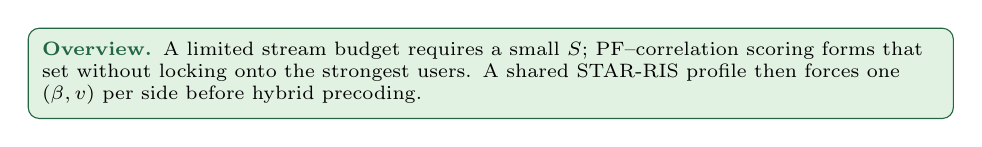
\begin{tikzpicture}
    \node[draw=notegreen, rounded corners, fill=softgreen,
          align=left, inner sep=5pt, text width=0.94\textwidth, font=\scriptsize] {
      \textbf{\color{notegreen}Overview.}
      A limited stream budget requires a small $S$; PF--correlation
      scoring forms that set without locking onto the strongest users.
      A shared STAR-RIS profile then forces one $(\beta,v)$ per side
      before hybrid precoding.};
  \end{tikzpicture}

  \vspace{-0.35cm}
  \begin{center}
  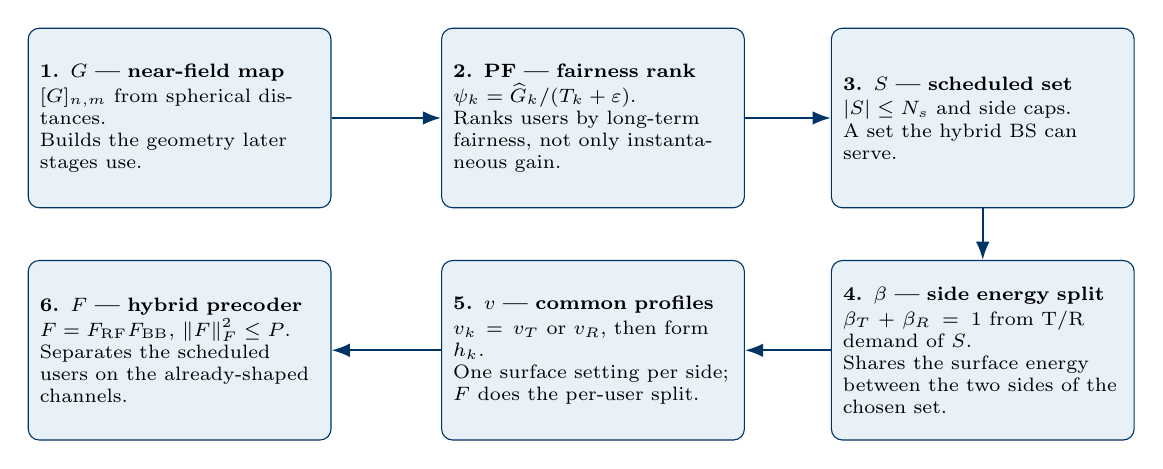
\begin{tikzpicture}[
      arr/.style={-{Latex}, thick, navyblue},
      card/.style={draw=navyblue, rounded corners, fill=softblue,
                   align=left, inner sep=4.2pt, font=\scriptsize,
                   text width=3.55cm, minimum height=2.28cm}
    ]
    % top: 1 2 3   (spread across the frame)
    \node[card] (c1) at (0,1.60) {%
      \textbf{1. $G$ --- near-field map}\\[0.12em]
      $[G]_{n,m}$ from spherical distances.\\
      Builds the geometry later stages use.};
    \node[card] (c2) at (5.25,1.60) {%
      \textbf{2. PF --- fairness rank}\\[0.12em]
      $\psi_k=\widehat{G}_k/(T_k+\varepsilon)$.\\
      Ranks users by long-term fairness,
      not only instantaneous gain.};
    \node[card] (c3) at (10.20,1.60) {%
      \textbf{3. $S$ --- scheduled set}\\[0.12em]
      $|S|\le N_s$ and side caps.\\
      A set the hybrid BS can serve.};
    % bottom: 6 5 4
    \node[card] (c6) at (0,-1.35) {%
      \textbf{6. $F$ --- hybrid precoder}\\[0.12em]
      $F=F_{\mathrm{RF}}F_{\mathrm{BB}}$, $\|F\|_F^2\le P$.\\
      Separates the scheduled users
      on the already-shaped channels.};
    \node[card] (c5) at (5.25,-1.35) {%
      \textbf{5. $v$ --- common profiles}\\[0.12em]
      $v_k=\vT$ or $\vR$, then form $h_k$.\\
      One surface setting per side;
      $F$ does the per-user split.};
    \node[card] (c4) at (10.20,-1.35) {%
      \textbf{4. $\beta$ --- side energy split}\\[0.12em]
      $\beta_T+\beta_R=1$ from T/R demand of $S$.\\
      Shares the surface energy between
      the two sides of the chosen set.};

    \draw[arr] (c1)--(c2);
    \draw[arr] (c2)--(c3);
    \draw[arr] (c3)--(c4);
    \draw[arr] (c4)--(c5);
    \draw[arr] (c5)--(c6);
  \end{tikzpicture}
  \end{center}
\end{frame}

%======================================================================
% PROPOSED --- RC-BDP: notice eqs, then bold-title colored boxes
%======================================================================
\begin{frame}{4. Proposed GA-HBF-PFBDP Scheme}
  \vspace{0.2cm}
  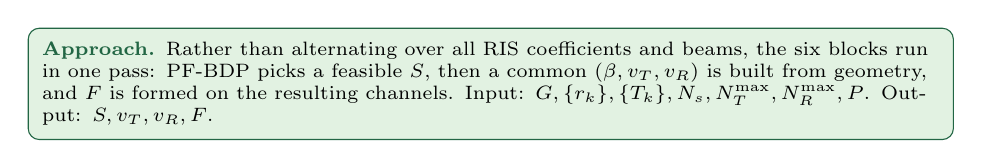
\begin{tikzpicture}
    \node[draw=notegreen, rounded corners, fill=softgreen,
          align=left, inner sep=5pt, text width=0.94\textwidth, font=\scriptsize] {
      \textbf{\color{notegreen}Approach.}
      Rather than alternating over all RIS coefficients and beams,
      the six blocks run in one pass: PF-BDP picks a feasible $S$,
      then a common $(\beta,\vT,\vR)$ is built from geometry, and $F$ is formed
      on the resulting channels.
      Input: $G,\{r_k\},\{T_k\},N_s,N_T^{\max},N_R^{\max},P$.
      Output: $S,\vT,\vR,F$.};
  \end{tikzpicture}

  \vspace{-0.35cm}
  \begin{center}
  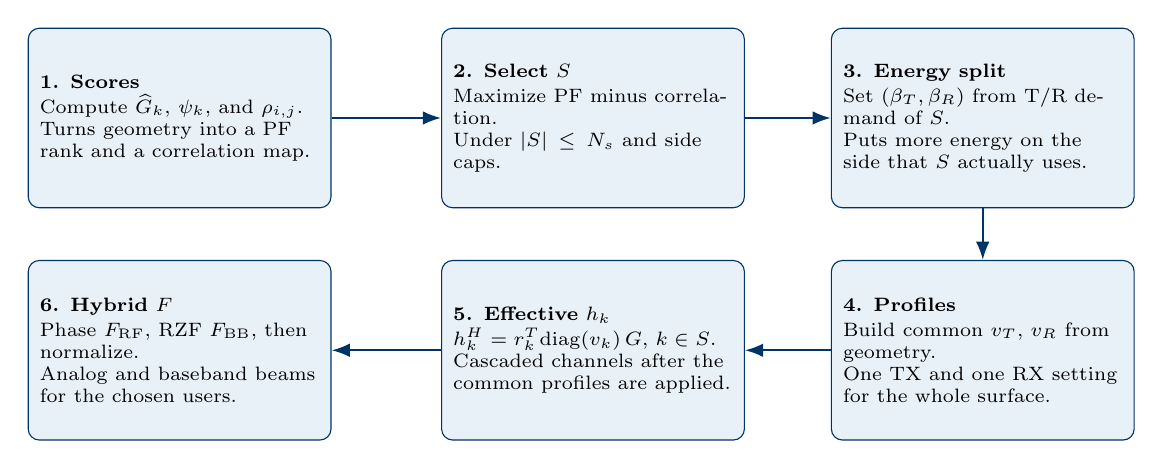
\begin{tikzpicture}[
      arr/.style={-{Latex}, thick, navyblue},
      card/.style={draw=navyblue, rounded corners, fill=softblue,
                   align=left, inner sep=4.2pt, font=\scriptsize,
                   text width=3.55cm, minimum height=2.28cm}
    ]
    \node[card] (c1) at (0,1.60) {%
      \textbf{1. Scores}\\[0.12em]
      Compute $\widehat{G}_k$, $\psi_k$, and $\rho_{i,j}$.\\
      Turns geometry into a PF rank
      and a correlation map.};
    \node[card] (c2) at (5.25,1.60) {%
      \textbf{2. Select $S$}\\[0.12em]
      Maximize PF minus correlation.\\
      Under $|S|\le N_s$ and side caps.};
    \node[card] (c3) at (10.20,1.60) {%
      \textbf{3. Energy split}\\[0.12em]
      Set $(\beta_T,\beta_R)$ from T/R demand of $S$.\\
      Puts more energy on the side
      that $S$ actually uses.};
    \node[card] (c6) at (0,-1.35) {%
      \textbf{6. Hybrid $F$}\\[0.12em]
      Phase $F_{\mathrm{RF}}$, RZF $F_{\mathrm{BB}}$, then normalize.\\
      Analog and baseband beams
      for the chosen users.};
    \node[card] (c5) at (5.25,-1.35) {%
      \textbf{5. Effective $h_k$}\\[0.12em]
      $h_k^H=r_k^T\mathrm{diag}(v_k)\,G$, $k\in S$.\\
      Cascaded channels after the
      common profiles are applied.};
    \node[card] (c4) at (10.20,-1.35) {%
      \textbf{4. Profiles}\\[0.12em]
      Build common $\vT$, $\vR$ from geometry.\\
      One TX and one RX setting
      for the whole surface.};

    \draw[arr] (c1)--(c2);
    \draw[arr] (c2)--(c3);
    \draw[arr] (c3)--(c4);
    \draw[arr] (c4)--(c5);
    \draw[arr] (c5)--(c6);
  \end{tikzpicture}
  \end{center}
\end{frame}

%======================================================================
% SIMULATION --- paper captions only, no extra comments
%======================================================================
\begin{frame}{5. Simulation Results (Rate)}
  \begin{columns}[T,onlytextwidth]
    \begin{column}{0.48\textwidth}
      \centering
      
\includegraphics[width=0.99\linewidth]{fig1.pdf}\\[0.15em]
      {\scriptsize Figure 1. Average sum-rate versus SNR for different beamforming schemes
      in a large STAR-RIS near-field system.}
    \end{column}
    \begin{column}{0.48\textwidth}
      \centering
      
\includegraphics[width=0.99\linewidth]{fig2.pdf}\\[0.15em]
      {\scriptsize Figure 2. Average sum-rate versus the number of STAR-RIS elements for
      different beamforming schemes.}
    \end{column}
  \end{columns}
\end{frame}

\begin{frame}{6. Simulation Results (Runtime and Users)}
  \begin{columns}[T,onlytextwidth]
    \begin{column}{0.48\textwidth}
      \centering
      
\includegraphics[width=0.99\linewidth]{fig3.pdf}\\[0.15em]
      {\scriptsize Figure 3. Average runtime per drop versus the number of STAR-RIS elements
      for different beamforming schemes.}
    \end{column}
    \begin{column}{0.48\textwidth}
      \centering
      
\includegraphics[width=0.99\linewidth]{fig4.pdf}\\[0.15em]
      {\scriptsize Figure 4. Average sum-rate versus the total number of users for different
      beamforming schemes.}
    \end{column}
  \end{columns}
\end{frame}

%======================================================================
% REFERENCES --- RC-BDP / CICN form: unnumbered IEEE, no extra title line
%======================================================================
\begin{frame}{7. References}
\fontsize{6.1pt}{7.15pt}\selectfont
\begin{thebibliography}{11}
\bibitem{elmossallamy}
M.~A.~ElMossallamy, H.~Zhang, L.~Song, K.~G.~Seddik, Z.~Han, and G.~Y.~Li,
``Reconfigurable intelligent surfaces for wireless communications: Principles, challenges, and opportunities,''
\textit{IEEE Trans.\ Cogn.\ Commun.\ Netw.}, vol.~6, no.~3, pp.~990--1002, 2020.
\bibitem{yuan_ris}
X.~Yuan, Y.-J.~A.~Zhang, Y.~Shi, W.~Yan, and H.~Liu,
``Reconfigurable-intelligent-surface empowered wireless communications: Challenges and opportunities,''
\textit{IEEE Wireless Commun.}, vol.~28, no.~2, pp.~136--143, 2021.
\bibitem{niu_star}
H.~Niu, Z.~Chu, F.~Zhou, P.~Xiao, and N.~Al-Dhahir,
``Simultaneous transmission and reflection reconfigurable intelligent surface assisted MIMO systems,'' 2021. [Online].
\bibitem{liu_star}
Y.~Liu, J.~Xu, Z.~Wang, X.~Mu, J.~Zhang, and P.~Zhang,
``Simultaneously transmitting and reflecting (STAR) RISs for 6G: Fundamentals, recent advances, and future directions,''
\textit{Frontiers Inf.\ Technol.\ Electron.\ Eng.}, vol.~24, no.~12, pp.~1689--1707, 2023.
\bibitem{hu_lis}
S.~Hu, H.~Wang, and M.~C.~Ilter,
``Design of near-field beamforming for large intelligent surfaces,''
\textit{IEEE Trans.\ Wireless Commun.}, vol.~23, no.~1, pp.~762--774, 2024.
%\bibitem{liu_nf_survey}
%Y.~Liu, C.~Ouyang, Z.~Wang, J.~Xu, X.~Mu, and A.~L.~Swindlehurst,
%``Near-field communications: A comprehensive survey,''
\textit{IEEE Commun.\ Surveys Tuts.}, vol.~27, no.~3, pp.~1687--1728, 2025.
\bibitem{li_star_nf}
H.~Li, Y.~Liu, X.~Mu, Y.~Chen, Z.~Pan, and Y.~C.~Eldar,
``Near-field beamforming for STAR-RIS networks,'' 2023. [Online].
\bibitem{wmmse}
S.~S.~Christensen, R.~Agarwal, E.~de~Carvalho, and J.~M.~Cioffi,
``Weighted sum-rate maximization using weighted MMSE for MIMO-BC beamforming design,''
in \textit{Proc.\ IEEE ICC}, 2009, pp.~1--6.
\bibitem{meng_isac}
C.~Meng, D.~Ma, Z.~Wang, Y.~Liu, Z.~Wei, and Z.~Feng,
``Near-field hybrid beamforming design for modular XL-MIMO ISAC systems,''
\textit{IEEE Trans.\ Commun.}, vol.~73, no.~11, pp.~11840--11854, 2025.
\bibitem{liu_elaa}
M.~Liu, M.~Li, R.~Liu, and Q.~Liu,
``Dynamic hybrid beamforming designs for ELAA near-field communications,''
\textit{IEEE J.\ Sel.\ Areas Commun.}, vol.~43, no.~3, pp.~644--658, 2025.
\bibitem{le_bdp}
T.~V.~Le, K.~Lee, and N.~Cong Luong,
``Bitmask dynamic programming for user scheduling in multi-user MIMO mmWave systems,''
\textit{IEEE Commun.\ Lett.}, vol.~27, no.~12, pp.~3365--3369, 2023.
\end{thebibliography}
\end{frame}


\begin{frame}[plain]
\begin{tikzpicture}[remember picture, overlay]
    \fill[navyblue] (current page.south west) rectangle (current page.north east);
\end{tikzpicture}
\vspace{1.5cm}
\begin{center}
    \textcolor{white}{\Huge\textbf{Thank You}}\\[0.8cm]
   % \textcolor{white}{\Large Questions?}\\[2cm]
    \textcolor{white}{\small \confshort~$\bullet$~Quy Nhon}
\end{center}
\end{frame}


\end{document}
